MAVLink is a telemetry protocol designed and developed for unmanned vehicles and other low-bandwidth systems. The binary protocol is well suited for resource-constrained systems and deployed in two versions: v1.0 and v2.0. MAVLink v2.0 is backwards-compatible i.e. it can parse and send v1.0 data packets.
Telemetry data which is less critical is sent in multicast streams while critical protocols that effect the system configuration or require guaranteed delivery like the mission or parameter protocol are sent point-to-point with re-transmission. The format of MAVLink protocol has been illustated in Fig \ref{fig:mavlink}.

\begin{figure}[h]
    \centering
    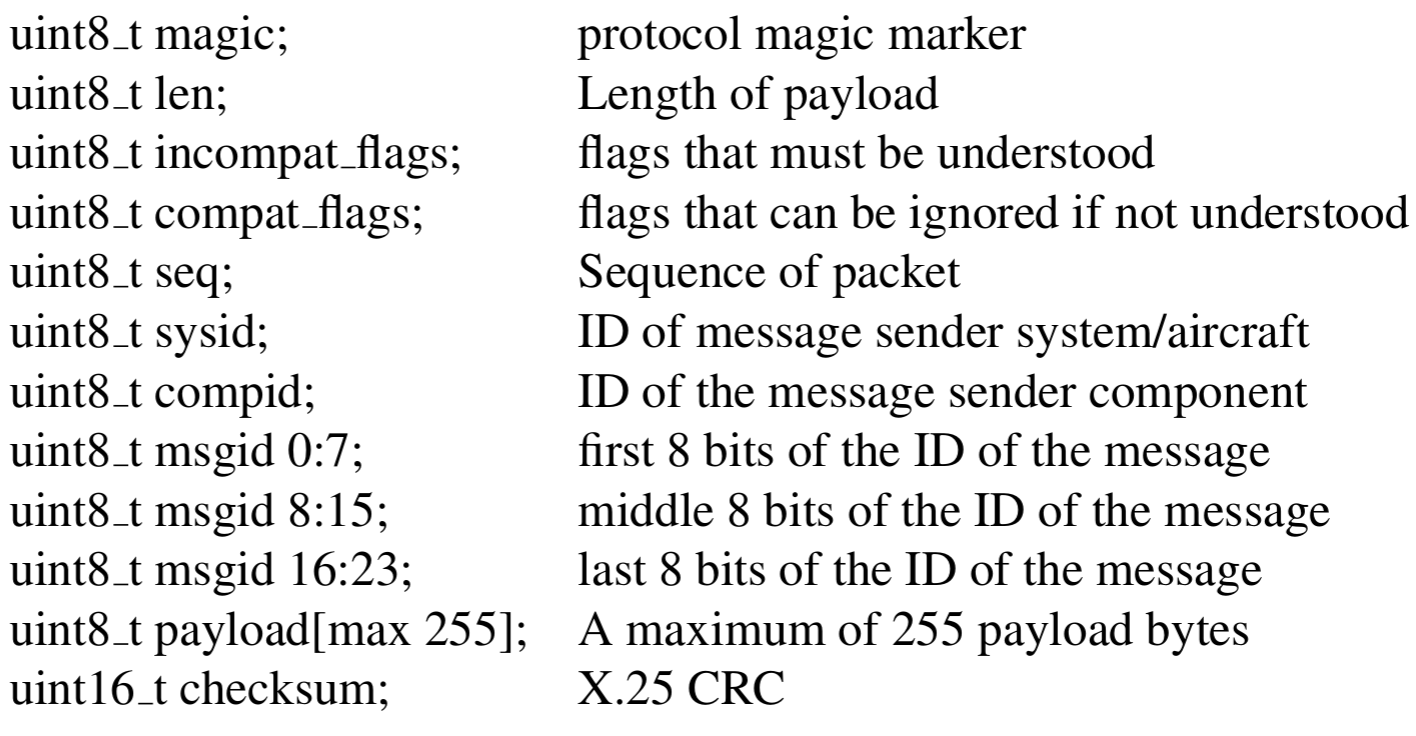
\includegraphics[width = 0.8\linewidth]{image/mavlinkprotocol.png}
    \caption{MAVLink Protocol Format}
    \label{fig:mavlink}
\end{figure}

\iffalse
\begin{table}[h]
    \centering
    \caption{MAVlink Protocol Format}
    \begin{tabular}{l l}
        uint8\_t magic; & protocol magic marker
\\uint8\_t len; & Length of payload
\\uint8\_t incompat\_flags;  &  flags that must be understood
\\uint8\_t compat\_flags;  &  flags that can be ignored if not understood
\\uint8\_t seq;  &  Sequence of packet
\\uint8\_t sysid;  &  ID of message sender system/aircraft
\\uint8\_t compid;  &  ID of the message sender component
\\uint8\_t msgid 0:7;  &  first 8 bits of the ID of the message
\\uint8\_t msgid 8:15;  &  middle 8 bits of the ID of the message
\\uint8\_t msgid 16:23;  &  last 8 bits of the ID of the message
\\uint8\_t payload[max 255];  &  A maximum of 255 payload bytes
\\uint16\_t checksum; &  X.25 CRC 
    \end{tabular}
    
    \label{tab:mavlink}
\end{table}
\fi